\documentclass{article}
\usepackage[utf8]{inputenc}
\usepackage[english]{babel}
\usepackage{graphicx}
\usepackage{float}

\begin{document}
\title{A Comparison of Dining Philosopher Solutions}
\author{Chris Dellomes\\
Professor: Carol LeDoux\\
CMSI 387: Operating Systems\\
	Loyola Marymount University}

\date{April 18, 2016}

\maketitle

\begin{center}
\begin{abstract}
This study is in response to the significance of the dining philosopher's problem in the field of operating systems. Synchronization and deadlock are important factors in the operating system development, which are simluated within the parameters of the problem. This paper presents comparative evaluations of three different solutions: Dijkstra's original solution, an arbitrator solution, and Chandy and Misra's cleanliness solution. Overall, the solution presented by Chandy andd Misra is the most effective of the three based on its scalability and efficiency.
\end{abstract}
\end{center}

\thispagestyle{empty}

\clearpage

\setcounter{page}{1}

\section{Introduction} The dining philosopher's problem is a significant point of discussion in the field of operating systems. It is a direct derivation of general issue of concurrent resource allocation, and thus the development of an efficient solution is a source of research and debate. The problem is defined as five philosophers at a table with five chopsticks between them to be used to eat. Each philosopher picks up each chopstick individually and is either in the process of eating or wating to eatThis paper will present a comparison of three distinct solutions and their overall effectiveness based on the criteria established by the problem's parameters. The problem was first proposed by Edsger Dijkstra, who developed an accompanying resource hierarchy algorithm for allocating the chopsticks amongst the philosophers. An alterante solution is to introduce an arbitrator entity, which moderates resource requests. In an attempt to improve upon previous solutions, Dr. Kanianthra Chandy and Dr. Jayadev Misra developed a solution in which resources are labeled as clean or dirty and are passed between requesting philosophers. Based on its scalability, lack of overhead, and safety, the solution developed by Chandy and Misra is the most effective and applicable to modern day operating systems.

\section{Background} The dining philosopher problem was originally invented by Dr. Edsger Dijkstra in 1965 as an exercise for his students. The problem was created to represent deadlock and starvation related problems in synchronization andd concurrent algorithm design. The problem was initially defined as five philosophers, who at anytime are either waiting or eating with five chopsticks between them. When a philosopher tries to eat, the philosopher picks up two chopsticks one at a time. The problem asks for a way to ensure every philosopher has the chance to eat. The solution avoids deadlock, but is slow to perform. After making the problem, Dijkstra proposed an accompanying solution in which each chopstick is numbered and each philosopher picks up the lower numbered chopsticks first. Following Dijkstra's creation of the problem and his initial solution, another solution surfaced which involves a waiter that regulates when philosophers can eat. The philosophers must ask the waiter if they are allowed to eat, after which the waiter checks to see if there are enough chopsticks available to satisfy the request, which results in an instruction to either take the chopsticks and eat or to continue waiting. The solution avoids deadlock, but reduces concurrent performance. In 1984, Dr. Kanianthra Chandy and Dr. Jayadev Misra, professors at CalTech and UT Austin, respectively, cooperatively developed a solution which introduces a cleanliness traits to all chopsticks. The solution is scalable to an arbitrarily large number of philosophers and chopsticks and prevents deadlock as well as starvation. As time has progressed, so have the effectiveness of solutions.

\section{Problem Description} The dining philosopher problem is defined as five philosophers all sitting together at a round table with five chopsticks for all of them to use. Each philosopher is either eating or waiting to eat. In order to eat, a philosopher must pick up and use the chopsticks to the immediate right and left one at a time. After eating, the philosopher puts down each chopstick one at a time. The philosophers are also not allowed to speak to each other. The goal of any solution is to ensure that every philosopher has a chance to eat.

\begin{figure}[H]
\begin{center}
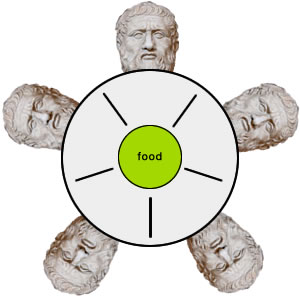
\includegraphics[width=0.3\textwidth]{diningphilosophers.jpg}
\caption{A visual representation of the dining philosopher's problem.}
\end{center}
\end{figure}

\section{Dijkstra's Solution} After creating and introducing the dining philosopher's problem to the field of computer science, Dijkstra presented his own solution based on establishing a hierarchy of resources. The chopsticks are ordered with each chopstick assigned a corresponding value.

\section{Conclusion}

\begin{thebibliography}{100}

\end{thebibliography}

\end{document}